{
\subsection{Opbygning af en Kørsel}
Start.py er distributør af arbejde til de andre dele af programkoden.
Her følger en kort beskrivelse af hvad start.py gør og derefter kan ses
noget pseudokode for hvad gør.
Når en ny kørsel skal laves, skal der laves en ny python fil i
eksperiments mappen og denne skal importeres som environment.
Når alle indstillinger globale eller kørsels afhængige er blevet sat,
startes analysen på et enkelt billede. Dette gentages indtil at alle
billederne er blevet analyseret.

\begin{lstlisting}
cuts = environment.generateCuts()
environment.setSettings(settings)
environment.setGlobalSettings(globalSettings)
db = Database(globalSettings)
run = m.createNewRun(settings)
paintings = m.Painting.select(m.Painting.q.form=="painting")
for painting in paintings:
	paintingContainer = Painting(painting)
	paintingContainer.setResults(paintingAnalyzer.analyze(paintingContainer,settings))
	m.saveResults(run.id,paintingContainer)
\end{lstlisting}
\begin{figure}[h!]
	\begin{center}
		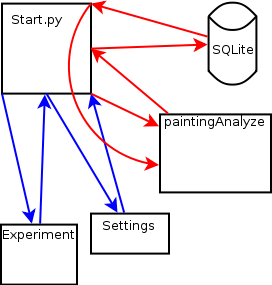
\includegraphics[scale=0.5]{afsnit/implementation/billeder/workflow_start_py.png}
	\end{center}
	\caption{De blå pile er ting, som sker en enkelt gang, mens de blå
	bliver gentaget indtil der ikke er flere billeder at arbejde på}
\end{figure}

\begin{lstlisting}[caption={Pseudokode for den naive metode},
    captionpos=b, label={pseudo_naiveMethod}, frame=tb,
    breaklines=false, float=h]
def NaiveMethod(image, settings):
    # Init ImageRegions dict
    ImageRegions = {}

    # Walk through all the CutRatios
    for CutRatio in settings:
        # Init RatioRegions dict
        RatioRegions = {}

        # Walk through every Cut in the ratio
        for Cut in CutRatio:
            # Set up the constraints, extract regions and prune the regions
            Constraints = new Constraints(image, Cut, settings)
            CutRegions = NaiveExtraction(image)
            InterestingRegions = GetInterestingRegions(CutRegions, Constraints)
            InterestingRegionsInCut =
                    GetInterestingRegionsInCut(InterestingRegionsInCut, Constraints)

            # Put the resulting instance of CutRegions
            # in the Regions-dict
            RatioRegions[Cut] = InterestingRegionsInCut

        # Put the resulting RatioRegions in the ImageRegions-dict
        ImageRegions[CutRatio] = RatioRegions

    # Return the resulting ImageRegions-dict
    return ImageRegions
\end{lstlisting}

\begin{lstlisting}[caption={Pseudokode til analyse af malerier efter
    metode}, captionpos=b, label={pseudo_naiveMethod}, frame=tb,
    breaklines=false, float=h]
def AnalysePainting(painting, settings):
    # Get the method used for the analysis
    method = settings.method

    # Use the right method
    if method == 'naive':
        image = painting.getImage()
        return NaiveMethod(image, settings)
    else:
        print 'No such method'
        return None
\end{lstlisting}

}
% vim: set tw=72 spell spelllang=da:
